\documentclass{ximera}
%% handout
%% nohints
%% space
%% newpage
%% numbers

%% You can put user macros here
%% However, you cannot make new environments

\graphicspath{{./}{firstExample/}{secondExample/}}

\usepackage{url}
\usepackage{tikz}
\usepackage{tkz-euclide}
\usetkzobj{all}


\tikzstyle geometryDiagrams=[ultra thick,color=blue!50!black]
\pgfplotsset{compat=1.8}
  \usepackage[T1]{fontenc}
  \usepackage[utf8x]{inputenc} %% we can turn off input when making a master document

\prerequisites{none}


\title{Introduction to Statistics}

\begin{document}
\begin{abstract}
We learn the basic terminology of statistics.
\end{abstract}
\maketitle

\subsection*{Basic learning objectives}

These are the tasks you should be able to perform with reasonable fluency \textbf{when you arrive at our next class meeting}. Important new vocabulary words are indicated \emph{in italics}. 

\begin{itemize}
    \item Understand the difference between \emph{probability} and \emph{statistics}.
    \item Understand how to organize data into a frequency table and to graph the distribution.
	\item Understand how to calculate the three \emph{measures of central tendency} of a list of data: \emph{mean}, \emph{median}, and \emph{mode}.
\end{itemize}

\subsection*{Advanced learning objectives}

In addition to mastering the basic objectives, here are the tasks you should be able to perform \textbf{after class, with practice}: 

\begin{itemize}
	\item Understand the distinction between having a sample of a population and having complete information on a population, and the dangers associated with inferring from a sample.
	\item Be able to calculate the three measures of central tendency from a frequency table.
    \item Be able to identify three typical shapes of distributions: normal, bimodal, and skewed.
\end{itemize}

\noindent\hrulefill

Probability and statistics are closely related concepts. They both often involve a sense of randomness about the information, but they start from two different places.

Probability starts with the assumption of a complete knowledge of all the possibilities and the chances of each event. For example, with a coin flipping experiment, we usually assume that the coin is fair, so that each side has a 50\% chance of landing face up. From that assumption, we can try to draw conclusions about what we expect to happen.

Statistics does not assume such information in advance. Instead, it looks at a \emph{sample} of the data (obtained by experiment, such as physically flipping a coin several times) and draws conclusions based on that information.

Suppose we have an urn that contains balls with numbers on them, but we don't know how many balls are in the urn nor what numbers are on the balls. Furthermore, we are restricted to only pulling out ten balls.

So we draw out the 10 balls one at a time (without replacement) and make a list of the numbers we see. The first ball has a 7, the second a 9, the third and fourth have an 8, the fifth is 10, and so on. We can turn this into a list.

\[ \{ 7, 9, 8, 8, 10, 7, 9, 8, 8, 8 \} \]

As a long list like this, the information is difficult to work with. We can turn the list into a \emph{frequency table} by keeping track of how many times we see each number.

\begin{image}
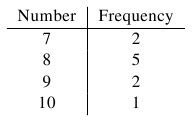
\includegraphics{StatsTable1.png}
%\begin{tikzpicture}
%\node(0,0){
%\begin{tabular}{c|c}
%Number & Frequency \\ \hline
%7 & 2 \\
%8 & 5 \\
%9 & 2 \\
%10 & 1
%\end{tabular}
%};
%\end{tikzpicture}
\end{image}

This information can also be turned into a bar graph:

\begin{image}
	\begin{tikzpicture}
		\begin{axis}[
        	ybar,
            enlargelimits=0.15,
            legend style={at={(0.5,-0.2)},
            anchor=north,legend columns=-1},
            ylabel={\# of Balls},
            symbolic x coords={7,8,9,10},
            xtick=data,
            nodes near coords,
            nodes near coords align={vertical},
            %x tick label style={rotate=45,anchor=east},
            ]
            
            \addplot coordinates {(7,2) (8,5) (9,2) (10,1)};
        \end{axis}
	\end{tikzpicture}
\end{image}

All of these are different ways of presenting the \emph{data set} we obtained by drawing balls from the urn. And now that we have the data, we can start to classify the information that we've obtained.

There are three pieces of information about numerical data that are collectively known as the \emph{measures of central tendency}: the mean, the median, and the mode.

The mean is what people generally mean when they talk about an average. It is calculated by adding up the values in the data set and dividing by the number of objects in the data set. Starting from the original list, we would get

\[ \text{mean} = \dfrac{7 + 9 + 8 + 8 + 10 + 7 + 9 + 8 + 8 + 8}{10} = 8.2. \]

The median is the number in the middle when arranged in order. When there is an odd number of data points, such as $[2, 5, 9]$, this is unambiguous (the median is 5). If there is an even number of data points, there is no middle number. In this case, we take the mean of the two middle-most numbers. This is the situation we have with the original data set:

\[ 7, 7, 8, 8, \underline{8} \underset{\uparrow}{,} \underline{8}, 8, 9, 9, 10 \rightarrow \text{median} = \dfrac{8 + 8}{2} = 8. \]

The mode is the number with the highest frequency. If there are multiple numbers that appear with the highest frequency, then we say that each of those numbers is a mode. For the data set above, the mode is 8.

\begin{question}
Which statement below is the correct?

    \begin{multipleChoice}
      \choice{Probability uses observed information and statistics uses assumed information.}
      \choice{Both probability and statistics use observed information.}
      \choice[correct]{Probability uses assumed information and statistics uses observed information.}
      \choice{Both probability and statistics use assumed information.}
    \end{multipleChoice}

\end{question} 

\begin{question}
Determine the mean of the following data set: $\{1, 1, 2, 5, 6\}$

    \begin{multipleChoice}
      \choice{1}
      \choice{2}
      \choice[correct]{3}
      \choice{4}
      \choice{5}
    \end{multipleChoice}
    \begin{hint}
      The mean is calculated by adding the numbers together and dividing by the number of data points.
    \end{hint}
    \begin{hint}
      This data set has 5 data points.
    \end{hint}

\end{question}

\begin{question}
Determine the median of the following data set: $\{32, 27, 40, 13, 18\}$

    \begin{multipleChoice}
      \choice{13}
      \choice[correct]{27}
      \choice{18}
      \choice{13}
      \choice{26}
      \choice{40}
    \end{multipleChoice}
    \begin{hint}
      Arrange the numbers in order.
    \end{hint}
    \begin{hint}
      The median is the middle number of the data set when the data set is put in order.
    \end{hint}

\end{question}

\begin{question}
Determine the mode of the following data set:
\begin{image}
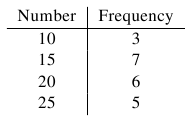
\includegraphics{StatsTable2.png}
%\begin{tikzpicture}
%\node(0,0){
%\begin{tabular}{c|c}
%Number & Frequency \\ \hline
%10 & 3 \\
%15 & 7 \\
%20 & 6 \\
%25 & 5
%\end{tabular}
%};
%\end{tikzpicture}
\end{image}


    \begin{multipleChoice}
      \choice{10}
      \choice[correct]{15}
      \choice{20}
      \choice{25}
    \end{multipleChoice}
    \begin{hint}
      The mode is the number with the highest frequency.
    \end{hint}

\end{question}

\end{document}